\subsection{Evaluation of SurroSelect on problems solved by third-party code}\label{sec:results-tool}
The tool was run on the eight \texttt{scikit-fem} problems at $N\in\{64,256,1024\}$ with three seeds (24 cells), and every pool member was also refit and scored on the 1000 test inputs, so that the \emph{oracle} (the best pool member by test error; unavailable in practice) is known. \Cref{tab:criteria} lists the pre-specified criteria and what was observed; \cref{tab:tperrors} gives the errors per problem. Only eight problems from four families are involved, and the three seeds of a problem share the pool and the test set, so cells are not independent; \cref{tab:criteria} therefore also gives problem-level intervals (resampling the eight problems), and the verdicts describe these eight problems only. The tuned network was run only at $N=256$ and $1024$ (16 cells); \cref{fig:strong} shows it next to the tool.
\begin{table}[t]\centering\caption{Pre-specified criteria (\cref{tab:hyp}) and results on the eight problems solved by third-party code. Intervals are 95\% (bootstrap for medians, Wilson for proportions, both treating cells as independent); problem-level intervals are in the text. The Holm-adjusted $p$-values are one-sided exact binomial tests against the thresholds.}\label{tab:criteria}\footnotesize\resizebox{\textwidth}{!}{\begin{tabular}{p{1.5cm}p{4.4cm}p{5.2cm}p{1.3cm}p{1.6cm}}
\toprule
ID & Criterion & Observed (95\% interval) & Holm $p$ & Verdict \\
\midrule
H1a & median regret $\le1.5$; $\ge75\%$ of cells $\le2$ & median 1.00 [1.00, 1.02]; 100\% [86\%, 100\%] & 0.003 & met \\
H1b & median ratio vs always-GP $\le1$ & 0.85 [0.59, 0.97]; better/worse 15/1 & -- & met \\
H1c & median ratio vs benchmark selection $\le1$; better $>$ worse & 1.01 [0.59, 1.19]; better/worse 11/9 & -- & not met \\
H2 & forecast within $\times2$ in $\ge70\%$ of 48 & 37 of 48 (77\% [63\%, 87\%]) & 0.363 & met \\
H2 (reach 1\%) & classification accuracy $\ge75\%$ & 100\% & -- & met \\
H2 (reach 0.1\%) & classification accuracy $\ge75\%$ & 88\% & -- & met \\
H3 & $\ge75\%$ of flagged cells (if $\ge5$) & 15 flagged; 15 better (100\%) & -- & met \\
H4 & strong network better by $>25\%$ in $\le4$ of 16 & 4 of 16 & 0.630 & met \\
H5 & reduced basis clear on $\ge5$ of 8 & 3 of 8 & -- & not met \\
\bottomrule
\end{tabular}
}\end{table}
\paragraph{Selection quality (H1a, H1b, H1c)} Cross-validated selection chose the oracle member in most cells, and the regret was at most \SoneMax{} in all \SoneN{} cells: median regret \SoneMedian{} (interval \SoneLo--\SoneHi), \SoneShare{} of cells within a factor two (Wilson interval \SoneWlo--\SoneWhi; H1a \SoneVerdict). Two caveats weaken this result. First, a fixed rule also passes the criterion: always choosing the single pool member \FixedBestName{} gives a median regret of \FixedBestRegret{} and puts \FixedBestShare{} of the cells within a factor two. The tool improves on that fixed choice by more than 10\% in \FixedBestBetter{} cells and loses by more than 10\% in \FixedBestWorse{} (median ratio \FixedBestRatio). Choosing a member at random would give a median regret of \NullRegret{} and \NullShare{} of cells within a factor two, so the tool is far from chance, but the fair reference is the best fixed member. Second, at the problem level, all eight problems have every cell within a factor two, yet a Wilson interval over eight problems has a lower limit of \PlSoneWlo, below the 75\% threshold; the problem-level interval of the median regret is \PlSoneLo--\PlSoneHi.
The tool was no worse than always using the benchmark's POD+GP (median ratio \StwoMedian, interval \StwoLo--\StwoHi, problem level \PlStwoLo--\PlStwoHi; better by more than 10\% in \StwoBetter{} cells, worse in \StwoWorse; H1b \StwoVerdict), which is nearly certain by construction because that model is a pool member. Against the benchmark's own selection among the five methods, which includes neural networks, the median ratio was \SthreeMedian{} (interval \SthreeLo--\SthreeHi, problem level \PlSthreeLo--\PlSthreeHi); the tool was better by more than 10\% in \SthreeBetter{} cells and worse in \SthreeWorse, so H1c is \textbf{\SthreeVerdict}. The cells where the tool loses (largest ratio \SthreeMaxRatio{} on \SthreeMaxWhere{}; \SthreeLshapeRatio{} on \texttt{lshape\_L2} at $N=1024$) are those in which a network from the benchmark beats every member of the default pool; the default pool contains no network.
\begin{table}[t]\centering\caption{Test error (geometric mean over three seeds) on the eight problems solved by third-party code: SurroSelect, the oracle (best pool member by test error), always POD+GP, the benchmark's validation-selected method, and the tuned network (only $N=256$ and $1024$).}\label{tab:tperrors}\scriptsize\resizebox{\textwidth}{!}{\begin{tabular}{lrrrrrr}
\toprule
Problem & N & Tool & Oracle & Always GP & Benchmark sel. & Tuned net \\
\midrule
\texttt{convdiff\_L1} & 256 & $4.2\times10^{-4}$ & $4.2\times10^{-4}$ & $1.6\times10^{-3}$ & $1.6\times10^{-3}$ & $2.4\times10^{-3}$ \\
\texttt{convdiff\_L2} & 256 & $1.1\times10^{-2}$ & $1.1\times10^{-2}$ & $1.5\times10^{-2}$ & $1.5\times10^{-2}$ & $1.1\times10^{-2}$ \\
\texttt{heatcomp\_L1} & 256 & $2.2\times10^{-3}$ & $2.0\times10^{-3}$ & $2.0\times10^{-3}$ & $2.0\times10^{-3}$ & $3.7\times10^{-3}$ \\
\texttt{heatcomp\_L2} & 256 & $1.6\times10^{-1}$ & $1.6\times10^{-1}$ & $1.9\times10^{-1}$ & $1.0\times10^{-1}$ & $1.2\times10^{-1}$ \\
\texttt{heatmove\_L1} & 256 & $9.0\times10^{-4}$ & $9.0\times10^{-4}$ & $7.5\times10^{-3}$ & $7.5\times10^{-3}$ & $5.5\times10^{-3}$ \\
\texttt{heatmove\_L2} & 256 & $2.1\times10^{-2}$ & $2.1\times10^{-2}$ & $3.2\times10^{-2}$ & $3.2\times10^{-2}$ & $2.7\times10^{-2}$ \\
\texttt{lshape\_L1} & 256 & $8.5\times10^{-4}$ & $8.5\times10^{-4}$ & $8.5\times10^{-4}$ & $8.5\times10^{-4}$ & $6.2\times10^{-3}$ \\
\texttt{lshape\_L2} & 256 & $7.6\times10^{-2}$ & $7.6\times10^{-2}$ & $7.4\times10^{-2}$ & $5.3\times10^{-2}$ & $3.7\times10^{-2}$ \\
\texttt{convdiff\_L1} & 1024 & $1.4\times10^{-5}$ & $1.4\times10^{-5}$ & $1.0\times10^{-3}$ & $1.0\times10^{-3}$ & $2.1\times10^{-3}$ \\
\texttt{convdiff\_L2} & 1024 & $1.9\times10^{-3}$ & $1.8\times10^{-3}$ & $8.3\times10^{-3}$ & $8.3\times10^{-3}$ & $5.6\times10^{-3}$ \\
\texttt{heatcomp\_L1} & 1024 & $1.2\times10^{-4}$ & $1.2\times10^{-4}$ & $4.3\times10^{-4}$ & $4.3\times10^{-4}$ & $2.1\times10^{-3}$ \\
\texttt{heatcomp\_L2} & 1024 & $8.1\times10^{-2}$ & $8.0\times10^{-2}$ & $9.0\times10^{-2}$ & $3.7\times10^{-2}$ & $3.6\times10^{-2}$ \\
\texttt{heatmove\_L1} & 1024 & $9.1\times10^{-5}$ & $9.1\times10^{-5}$ & $6.6\times10^{-3}$ & $4.5\times10^{-3}$ & $3.5\times10^{-3}$ \\
\texttt{heatmove\_L2} & 1024 & $4.2\times10^{-3}$ & $4.2\times10^{-3}$ & $2.1\times10^{-2}$ & $1.5\times10^{-2}$ & $1.3\times10^{-2}$ \\
\texttt{lshape\_L1} & 1024 & $7.1\times10^{-5}$ & $6.1\times10^{-5}$ & $1.2\times10^{-4}$ & $1.2\times10^{-4}$ & $3.6\times10^{-3}$ \\
\texttt{lshape\_L2} & 1024 & $2.8\times10^{-2}$ & $2.8\times10^{-2}$ & $2.5\times10^{-2}$ & $2.0\times10^{-2}$ & $1.7\times10^{-2}$ \\
\bottomrule
\end{tabular}
}\end{table}
\paragraph{Budget forecast (H2)} For the 48 cases, the forecast from $N_0$ runs of the error at $4N_0$ runs was within a factor two of the actual error in \BoneK{} (\BoneShare, Wilson interval \BoneLo--\BoneHi, problem level \PlBoneLo--\PlBoneHi; \BoneVerdict), but the interval includes the threshold of 70\% (one-sided exact binomial $p=\BonePRaw$ against it, Holm-adjusted \HolmBOneSevenZero). The pre-specified pooled criterion was met only because of the small budget: \BoneShareSixtyfour{} of the cases from $N_0=64$ but only \BoneWithinTwofiftysix{} of 24 (\BoneShareTwofiftysix) from $N_0=256$, which is below the threshold, and \BoneUnderTwofiftysix{} of the forecasts from 256 runs were too low by more than a factor two (\cref{fig:validity}). Overall \BoneUnder{} forecasts were too low and \BoneOver{} too high, and all misclassifications at the 0.1\% target were optimistic. Errors that fall faster than a power law over the last data points are extrapolated too optimistically. The range between the two fits contains the actual error in only \BoneBand{} of the cases and must not be read as an uncertainty interval. For the decision ``will 1\% (0.1\%) be reached at 1024 runs?'' from 256 runs, the forecast was right in \BtwoOneAcc{} (\BtwoTenthAcc) of 24 cases; always guessing the more common answer would be right in \BtwoOneMajor{} (\BtwoTenthMajor), so the 1\% result carries no information beyond the base rate and the 0.1\% result is above the base rate but not significant against the 75\% threshold (one-sided $p=\BtwoTenthP$).
\begin{figure}[t]\centering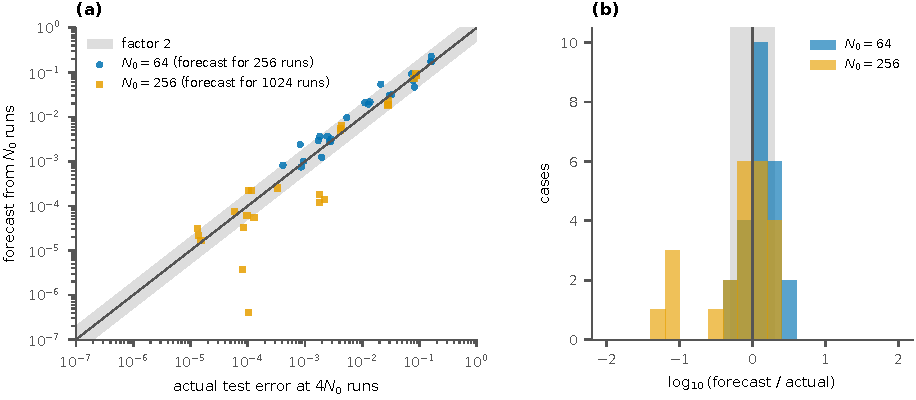
\includegraphics[width=\textwidth]{figures/fig_validity.pdf}
\caption{The learning-curve forecast is useful from small budgets and too optimistic from larger ones. (a) Forecast against actual test error at four times the starting budget (48 cases; problems solved by third-party code; shaded: within a factor two). (b) Histogram of $\log_{10}$(forecast/actual); cases below $-0.3$ are forecasts that are too low.}\label{fig:validity}\end{figure}
\paragraph{Basis check (H3)} The flag was raised in \HthreeJobs{} of the 72 fits, which are \HthreeCells{} distinct (problem, budget) cells from \HthreeProblems{} problems (convection--diffusion and transient heat); in all of them a full-field Gaussian process had a test error more than 10\% below the best POD-based member (H3 \FoneVerdict; the comparison is by test error over five POD members and two full-field members). This evidence is thinner than the count suggests. The flag was raised in only \HthreeRecall{} of the \HthreeFullJobs{} fits in which a full-field member was better by more than 10\%, so its recall is low, and in all \HthreeSelected{} flagged fits the cross-validated selection had already chosen a full-field member, so on these data the flag explained a decision rather than changed it. The flagged problems are those where the benchmark found networks competitive with the POD-based Gaussian process, which is consistent with \cref{prop:floor}.
\paragraph{Against a tuned network (H4)} The tuned network (Optuna, 16 trials; compared with the benchmark networks it also has four times the epochs, double precision and an L-BFGS polish, and about twice the trials) was better than the tool-selected model by more than 25\% in \SfourBetter{} of \SfourN{} cells (H4 \SfourVerdict, exactly at the limit of four). These \SfourBetter{} cells come from \StrongProblemsN{} problems (composite conduction and the L-shaped plate, both with seven or nine inputs, at two budgets each), and the Wilson interval for their share, \SfourWlo--\SfourWhi, is wide. The median ratio of the tool's error to the tuned network's was \SfourMedian; the tool was better by more than 10\% in \SfourToolBetter{} cells and the network in \SfourStrongBetter. The tuned network improved on the benchmark's networks in \StrongLegacyN{} of 16 cells (median error ratio \StrongLegacyRatio), but on the smooth problems at $N=1024$ its error was still up to \StrongWorstProblemRatio{} times that of the tool, so it is probably under-trained and H4 says little about what a well-tuned network could reach. It needed a median of \StrongSecTwofiftysix{}~s ($N=256$) and \StrongSecTentwentyfour{}~s ($N=1024$) on one core, against \ToolFitSecTwofiftysix{} and \ToolFitSecTentwentyfour{}~s for the tool's cross-validated selection (\cref{sec:cost}).
\begin{figure}[t]\centering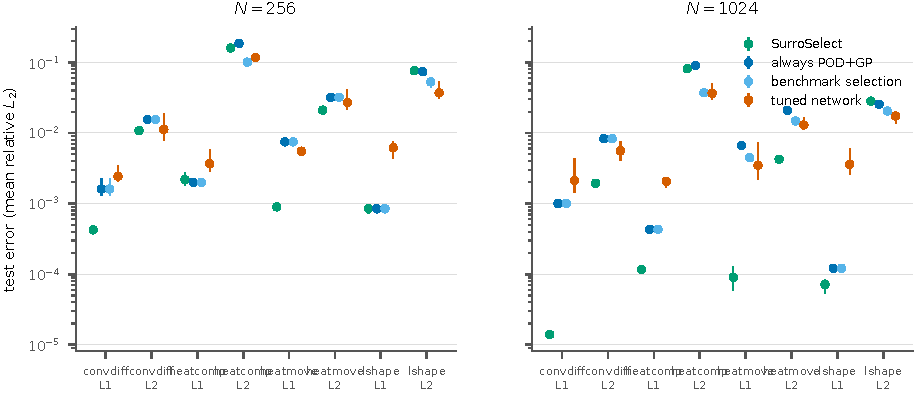
\includegraphics[width=\textwidth]{figures/fig_strong_nn.pdf}
\caption{Test error of the tool and its competitors on each problem solved by third-party code. Points: geometric mean over three seeds; bars: minimum to maximum over seeds. The tuned network was run at $N=256$ and $1024$ only.}\label{fig:strong}\end{figure}
The tool's advantage over the tuned network is largest on the smooth problems, and the network wins on the two problems with seven or nine inputs (\cref{fig:strong}).

\subsection{Ablation, noise and cost}\label{sec:cost}
\paragraph{Ablation} Restricting the pool, with selection by the stored cross-validation errors (\cref{tab:ablation}), shows which members matter: without the full-field Gaussian process the regret is within a factor two in only \AblPodonlyShare{} of cells, and without any Gaussian-process member (ridge and polynomial only) the test error is a median \AblNogpMedian{} times larger than with the full pool.
\begin{table}[t]\centering\caption{Ablation of the pool on the eight problems solved by third-party code (24 cells); regret as in \cref{sec:setup}.}\label{tab:ablation}\small\resizebox{\textwidth}{!}{\begin{tabular}{lrrr}
\toprule
Pool & Median regret & Cells with regret $\le2$ & Median error vs full pool \\
\midrule
full pool & 1.00 & 100\% & 1.00$\times$ \\
POD-based members only & 1.07 & 75\% & 1.02$\times$ \\
no full-field GP & 1.07 & 75\% & 1.02$\times$ \\
GP members only & 1.01 & 96\% & 1.00$\times$ \\
no GP (ridge, polynomial) & 2.81 & 33\% & 2.74$\times$ \\
\bottomrule
\end{tabular}
}\end{table}
\paragraph{Sampling noise} A pool member picked at random gives median regret \NullRegret, and the seed-to-seed spread of the tool's regret is small (median regret \SoneMedianSixtyfour, \SoneMedianTwofiftysix{} and \SoneMedianTentwentyfour{} at the three budgets), so the observed regrets are not explained by chance. Seeds share the pool and test set and nest their training subsets, so seed variability understates the variability of a new sample of runs.
\paragraph{Computational cost} Measured on \HwCores{} cores (\HwCpu), one thread per fit, selection with cross-validation took a median of \ToolFitSecSixtyfour{}, \ToolFitSecTwofiftysix{} and \ToolFitSecTentwentyfour{}~s at $N=64$, 256 and 1024; adding the learning curve brought this to \ToolTotalSecSixtyfour{}, \ToolTotalSecTwofiftysix{} and \ToolTotalSecTentwentyfour{}~s. The solvers of these problems take \TpFomLo--\TpFomHi~ms per run, so for them the tool costs more than running the simulation 1024 times; its use is justified when one run takes minutes or hours.
\paragraph{Complexity} Let $N$ be the number of runs, $m$ the number of outputs, $p$ the number of inputs, $r$ the number of POD modes and $k$ the number of folds. The dominant costs are: an exact Gaussian process with fixed hyper-parameters, $O(N^3+N^2 r)$ per fit; hyper-parameter fitting, which uses at most 300 runs and costs $O(n_{\rm opt}^3 p)$ per optimiser step on the leading modes; kernel ridge, one eigendecomposition per kernel and length-scale, $O(N^3)$ each, with the whole ridge grid scored in $O(N^2)$ each; the polynomial, one singular value decomposition of the $N\times F$ design matrix with $F\le3000$, $O(NF^2)$; the full-field Gaussian process, as the POD-based one with all $m$ outputs sharing one kernel, $O(N^3+N^2m)$; the POD, $O(Nm\min(N,m))$. Cross-validation multiplies each by $k$, and the learning curve adds about $\sum_j k\,c(N/2^j)$, i.e.\ roughly one further cross-validated fit of the selected member. Between $N=256$ and $1024$ the measured median selection time grew by a factor of about \ToolScaleRatio, against the factor 64 predicted by cubic scaling, because the hyper-parameter fit is capped at 300 runs.

\subsection{Qualitative analysis}\label{sec:qualitative}
\Cref{fig:qual} shows the first test sample in dataset order for the first problem of each family at $N=256$ (seed 0), and failure cases selected by rules fixed before the figure was made: the problem with the largest selection regret at $N=256$ and the problem with the largest test error (a problem that is already shown is not repeated). The selected model reproduces the large-scale structure of the fields in the rule-selected examples, with relative errors given beside each panel; the error maps show structure rather than noise, so the remaining error is systematic. In the failure case with the largest error (the nine-input, high-contrast composite-conduction problem) the error is spread over the whole field, so no member of the pool captures this map at 256 runs; this is consistent with the benchmark, where networks beat the reduced-basis group on this problem.
\begin{figure}[t]\centering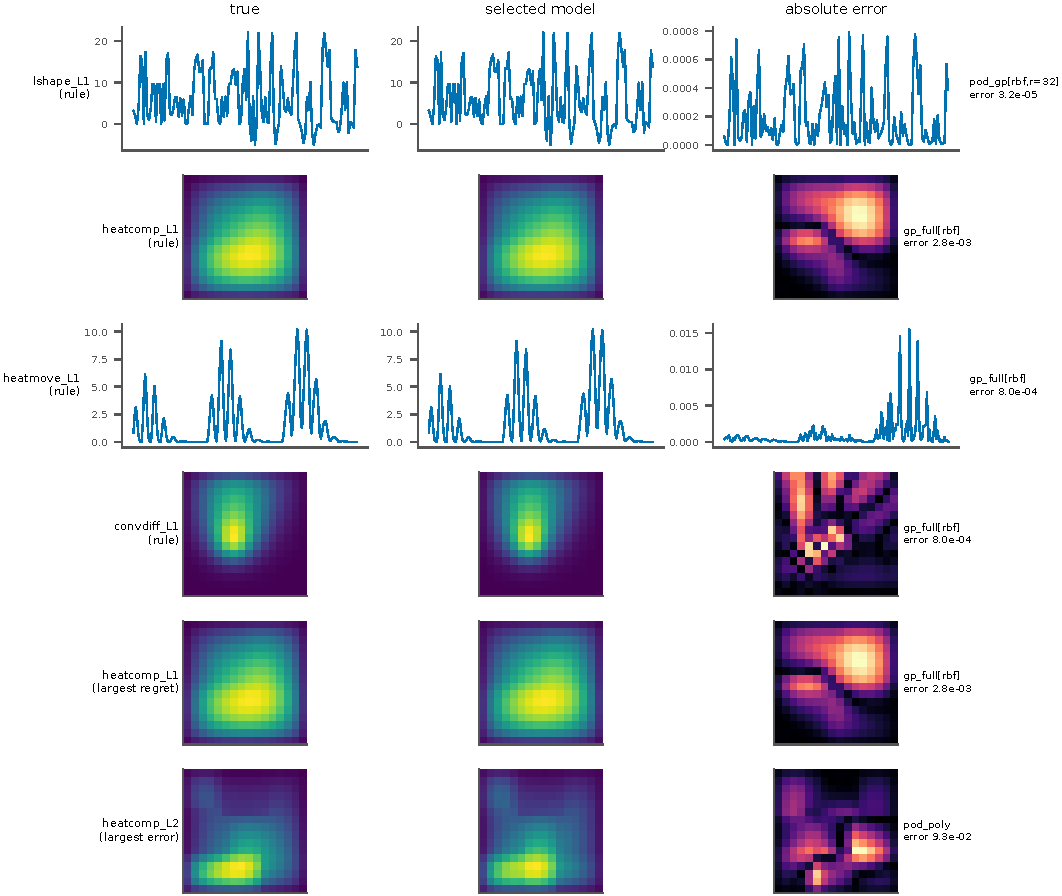
\includegraphics[width=0.9\textwidth]{figures/fig_qualitative.pdf}
\caption{The selected model reproduces the large-scale structure of single test fields; its errors are systematic. Predictions of the selected model on single test samples chosen by a fixed rule (first test sample in dataset order, first problem of each family, plus the failure cases defined in \cref{sec:qualitative}). Columns: true field, selected model, absolute error; the L-shaped plate has no regular grid and is shown as a profile over probe nodes.}\label{fig:qual}\end{figure}

\subsection{Comparative analysis and real-data check}\label{sec:real}
\paragraph{Comparison with the benchmark} Together with \cref{sec:results-study}: on smooth problems with few inputs a Gaussian-process or well-regularised kernel member of the pool is hard to beat; where the POD basis limits accuracy a full-field Gaussian process is the better choice; and where networks from the benchmark win (the composite-conduction problem with nine inputs), the default pool cannot match them (H1c). The tool's contribution is to find these cases from the training runs alone. In a descriptive, design-informed run on the 36 earlier problems (one seed, $N=256$; Supplement, Sec.~\ref{sec:S-retro}), the tool's selection can be compared with the oracle, but those problems were used to design the pool and the run is not evidence for the criteria.
\paragraph{Real measured data} Two real datasets were used (\texttt{data\_real/}, CC BY 4.0): wind-tunnel measurements of airfoil noise (1,503 rows, five inputs) and the output of a combined-cycle power plant (9,568 rows, four inputs). Both have a scalar, noisy output, so they violate assumption A2, are not field data, and make the POD rank one, so the data say nothing about the POD-versus-full-field choice that the tool is built around; the normalised RMSE replaces the relative error. With the protocol of Supplement addendum v3.1 (committed before any model was fitted to these data), median regret was \RealRoneMedian{} over six cells (R1 \RealRoneVerdict), the tool was no worse than always-POD+GP in \RealRtwoK{} of \RealRtwoN{} cells (R2 \RealRtwoVerdict; two of the successes are exact ties, because the same model was chosen), the tuned network was better by more than 25\% in \RealRthreeK{} cells (R3 \RealRthreeVerdict), and \RealRfourK{} of \RealRfourN{} forecasts were within a factor two (R4 \RealRfourVerdict). We had predicted that R4 would fail because of measurement noise; it did not. The airfoil pool holds only 1,052 rows, so its $N=1024$ results use nearly all of it. \Cref{tab:real} lists the errors.
\begin{table}[t]\centering\caption{Real-data check: normalised RMSE of the tool, the oracle, always-POD+GP and the tuned network (geometric mean over three seeds).}\label{tab:real}\small\resizebox{\textwidth}{!}{\begin{tabular}{lrrrrrr}
\toprule
Dataset & N & Tool & Oracle & Always GP & Tuned net & Regret \\
\midrule
airfoil & 64 & 0.5960 & 0.5218 & 0.5868 & 0.6792 & 1.14 \\
airfoil & 256 & 0.3585 & 0.3578 & 0.3585 & 0.4072 & 1.00 \\
airfoil & 1024 & 0.2107 & 0.1845 & 0.2107 & 0.2037 & 1.14 \\
ccpp & 64 & 0.2867 & 0.2676 & 0.3153 & 0.5854 & 1.07 \\
ccpp & 256 & 0.2554 & 0.2539 & 0.2920 & 0.3682 & 1.01 \\
ccpp & 1024 & 0.2453 & 0.2437 & 0.2500 & 0.3530 & 1.01 \\
\bottomrule
\end{tabular}
}\end{table}
\paragraph{Plain-file validation and case study} The three command-line commands were run on exported files for three problems; all sequences ran, and the error printed by \texttt{evaluate} matched an independent computation (Supplement, Sec.~\ref{sec:S-tool}). \Cref{lst:case} shows the report for problem \texttt{heatmove\_L1} with 256 runs and a target error of 0.1\%.
\begin{figure}[t]\centering\small
\begin{minipage}{0.95\textwidth}\scriptsize\verbatiminput{tables/case_report_wrapped.txt}\end{minipage}
\caption{SurroSelect report (in Markdown) for \texttt{heatmove\_L1} (256 runs, seed 0, target error 0.1\%), unedited except for line wrapping.}\label{lst:case}\end{figure}
